\chapter{Introduction}

% Present the kind of problems we're going to work on, and sketch the way.

An equation that models an evolution process that contains `noise', with a certain randomness, is an equation of the form:
\begin{equation}\label{eq:sde}
	\frac{\, \mathrm{d}X}{\, \mathrm{d}t} = b(t,X_t) + \sigma(t,X_t)\cdot \text{`white noise'}
\end{equation}

Problems like this appears naturally in biology (populational growth models), physics (charge in electrical circuits), engineering (filtering problems, like the Kalman's Filter exihibted in the Figure \ref{fig:kalman}) and finance (optimal stopping, optimal portfolio and option pricing).

\begin{figure}[h]
  \centering
    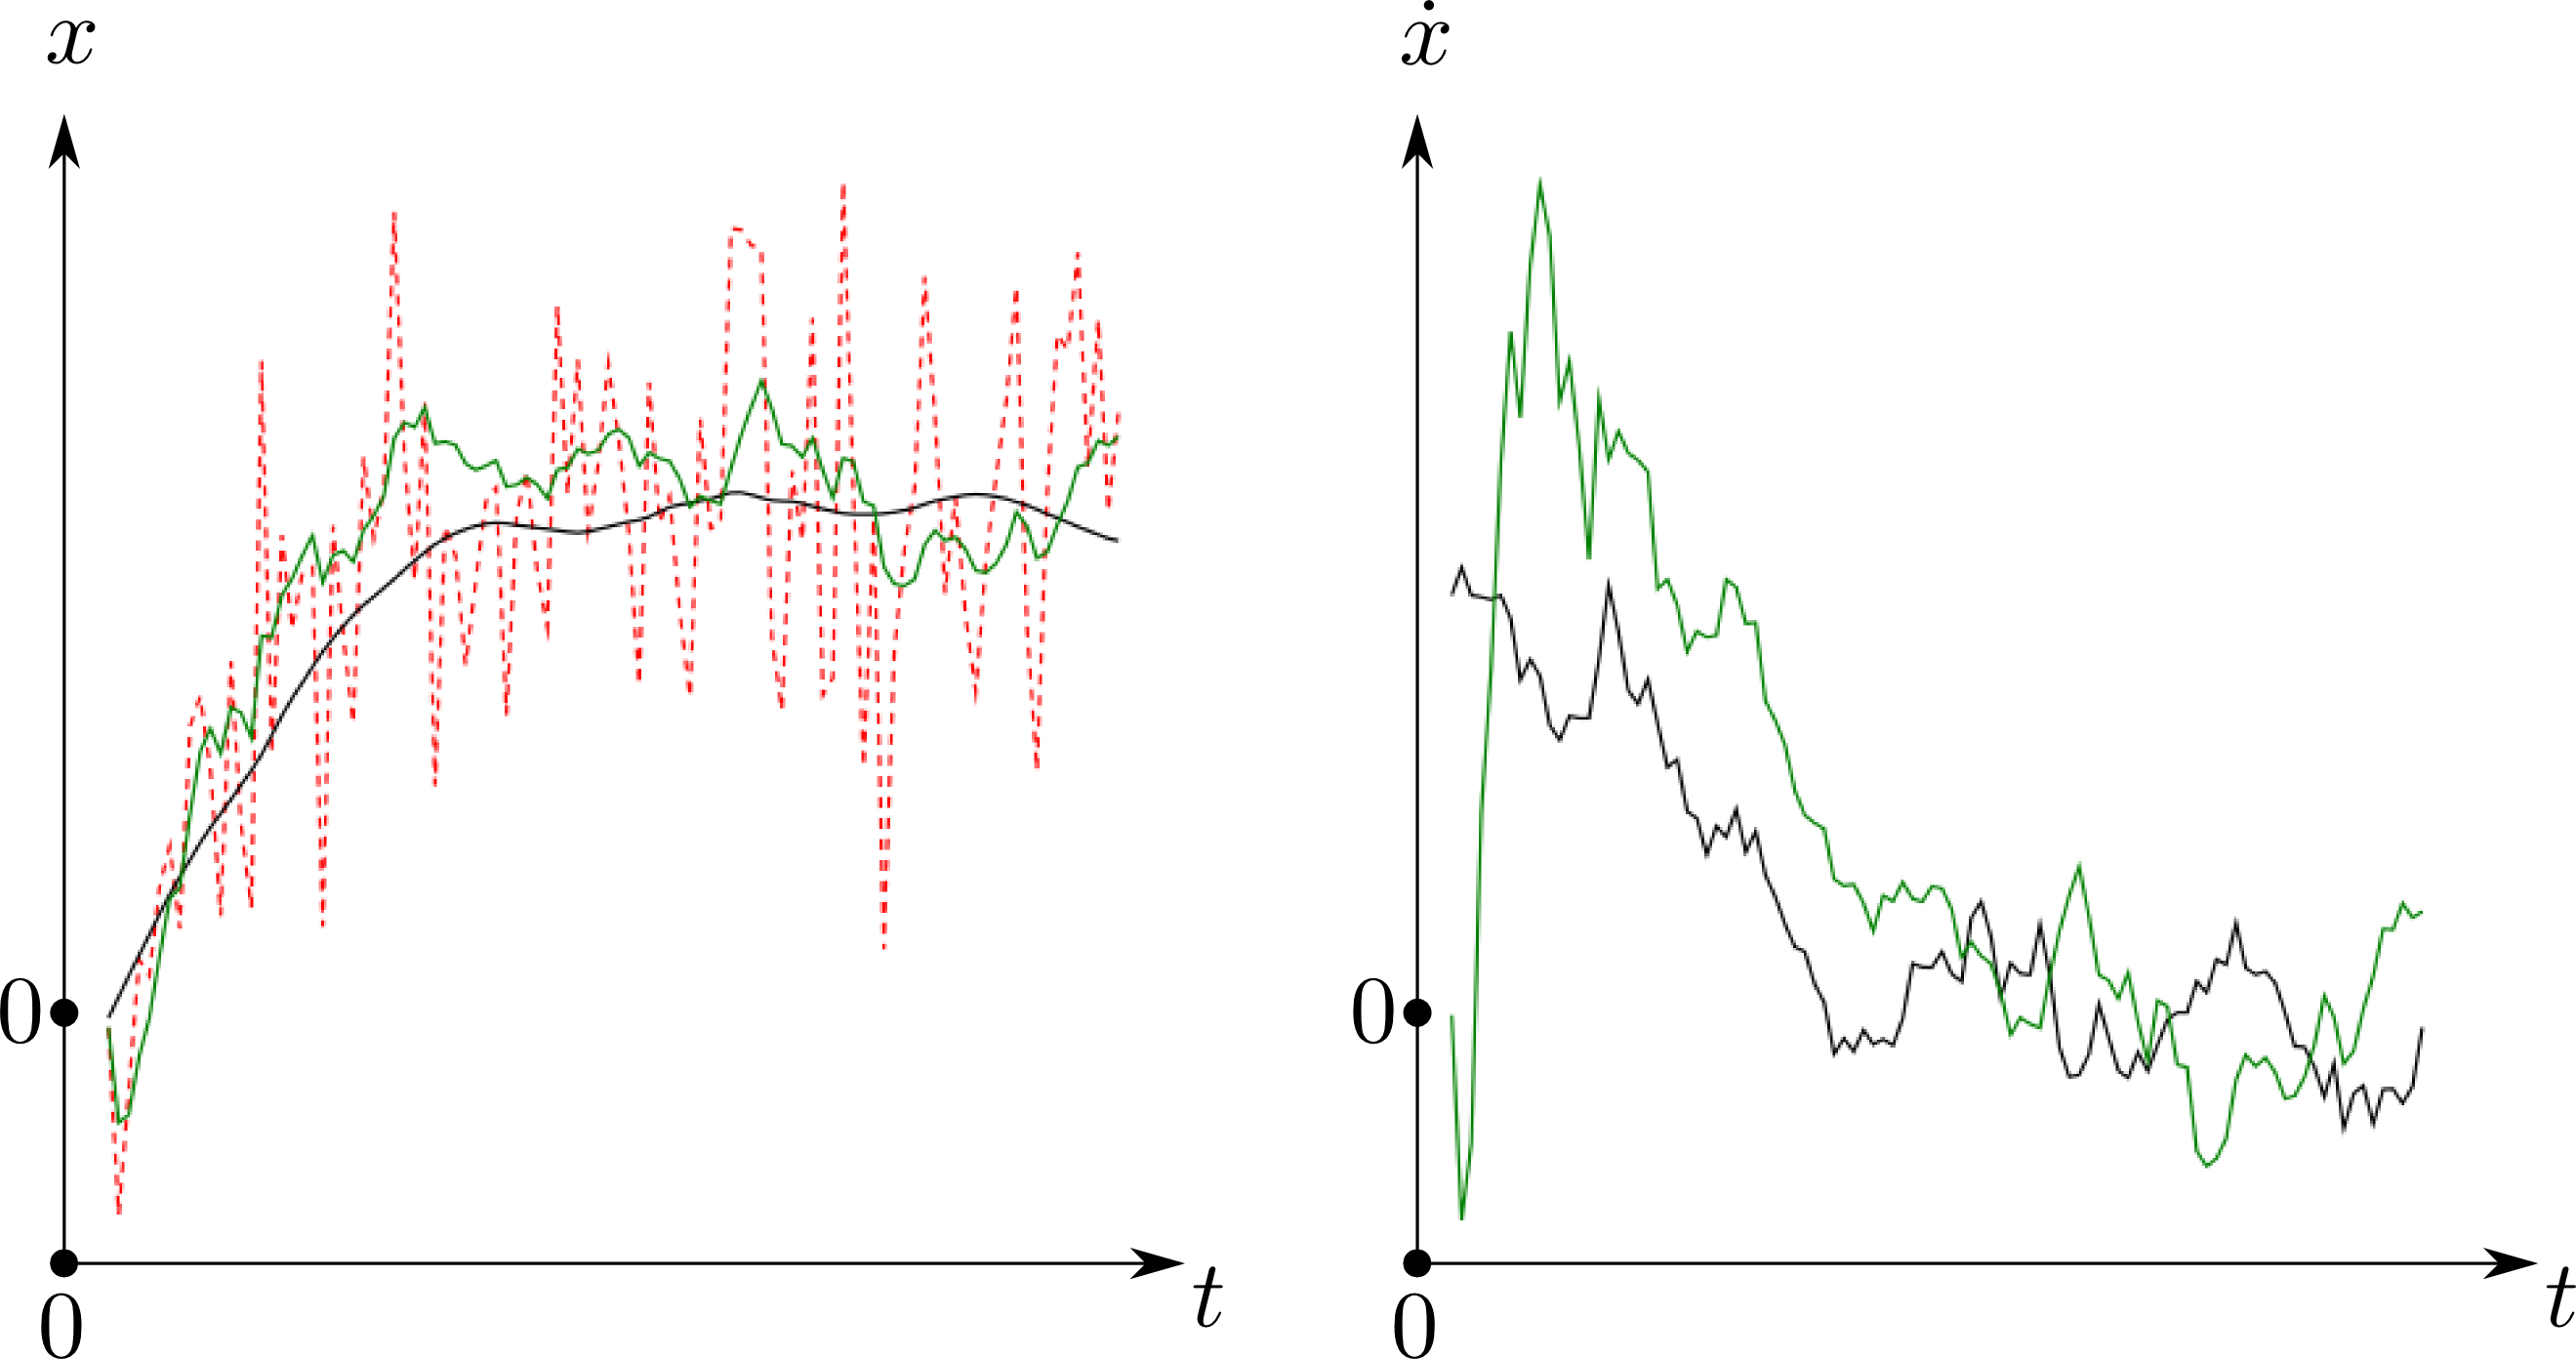
\includegraphics[width=0.7\textwidth]{Figures/Kalman.png} 
    \caption{Kalman's Filter: $\crule[red]{0.4cm}{0.4cm}$ Observed data; $\crule[ForestGreen]{0.4cm}{0.4cm}$ Filtered process; $\crule{0.4cm}{0.4cm}$ Real data \cite{wiki:Kalman_filter}.}
    \label{fig:kalman}
\end{figure}

From the mathematical viewpoint, we need to make sense of this kind of equations, since with the usual tools of calculus, it is not possible to treat them. Our goal then, in this work, is to give the foundations that allow us to treat this equations. In particular, firstly we're going to define the Itô's Integral and then we'll be ready to tackle stochastic differential equations.